\section{Logger Class Reference}
\label{classLogger}\index{Logger@{Logger}}
Inheritance diagram for Logger:\begin{figure}[H]
\begin{center}
\leavevmode
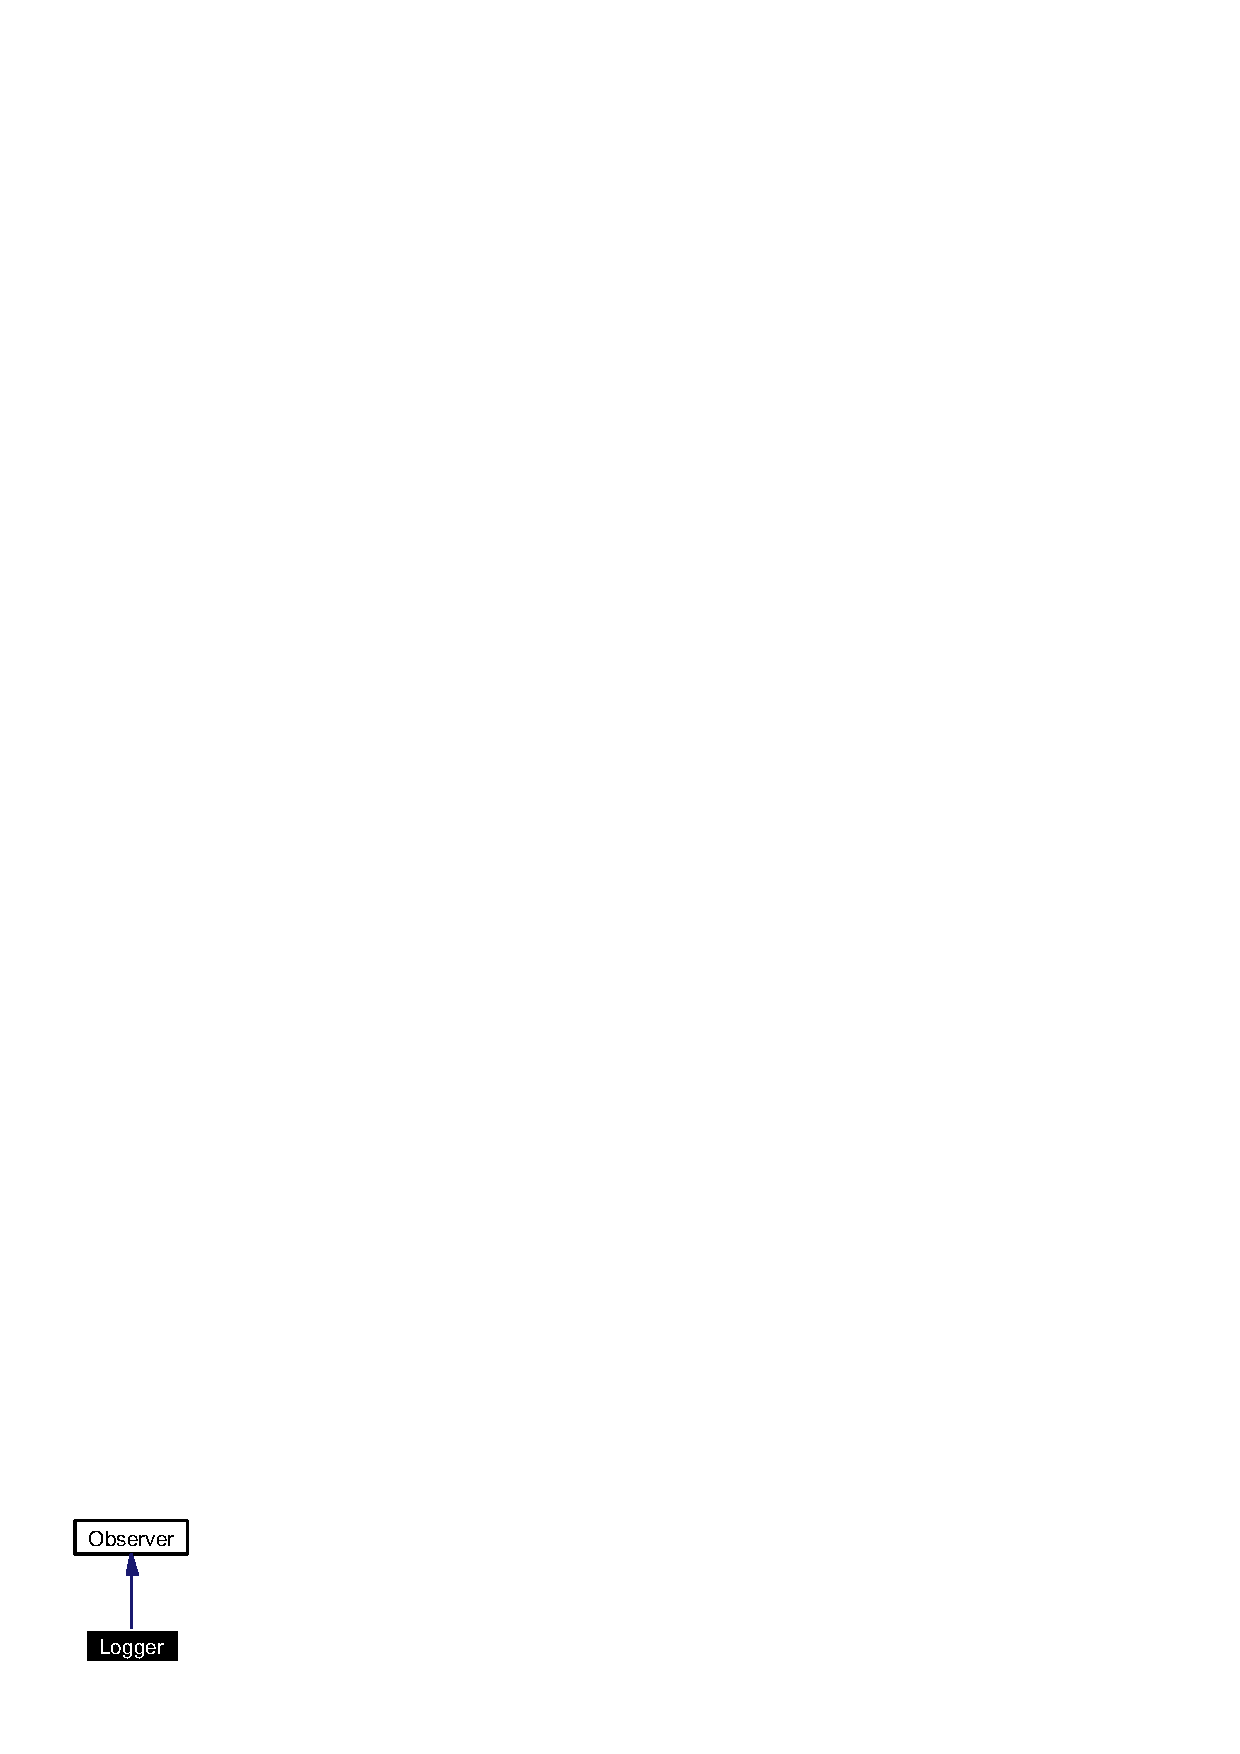
\includegraphics[width=45pt]{classLogger__inherit__graph}
\end{center}
\end{figure}
Collaboration diagram for Logger:\begin{figure}[H]
\begin{center}
\leavevmode
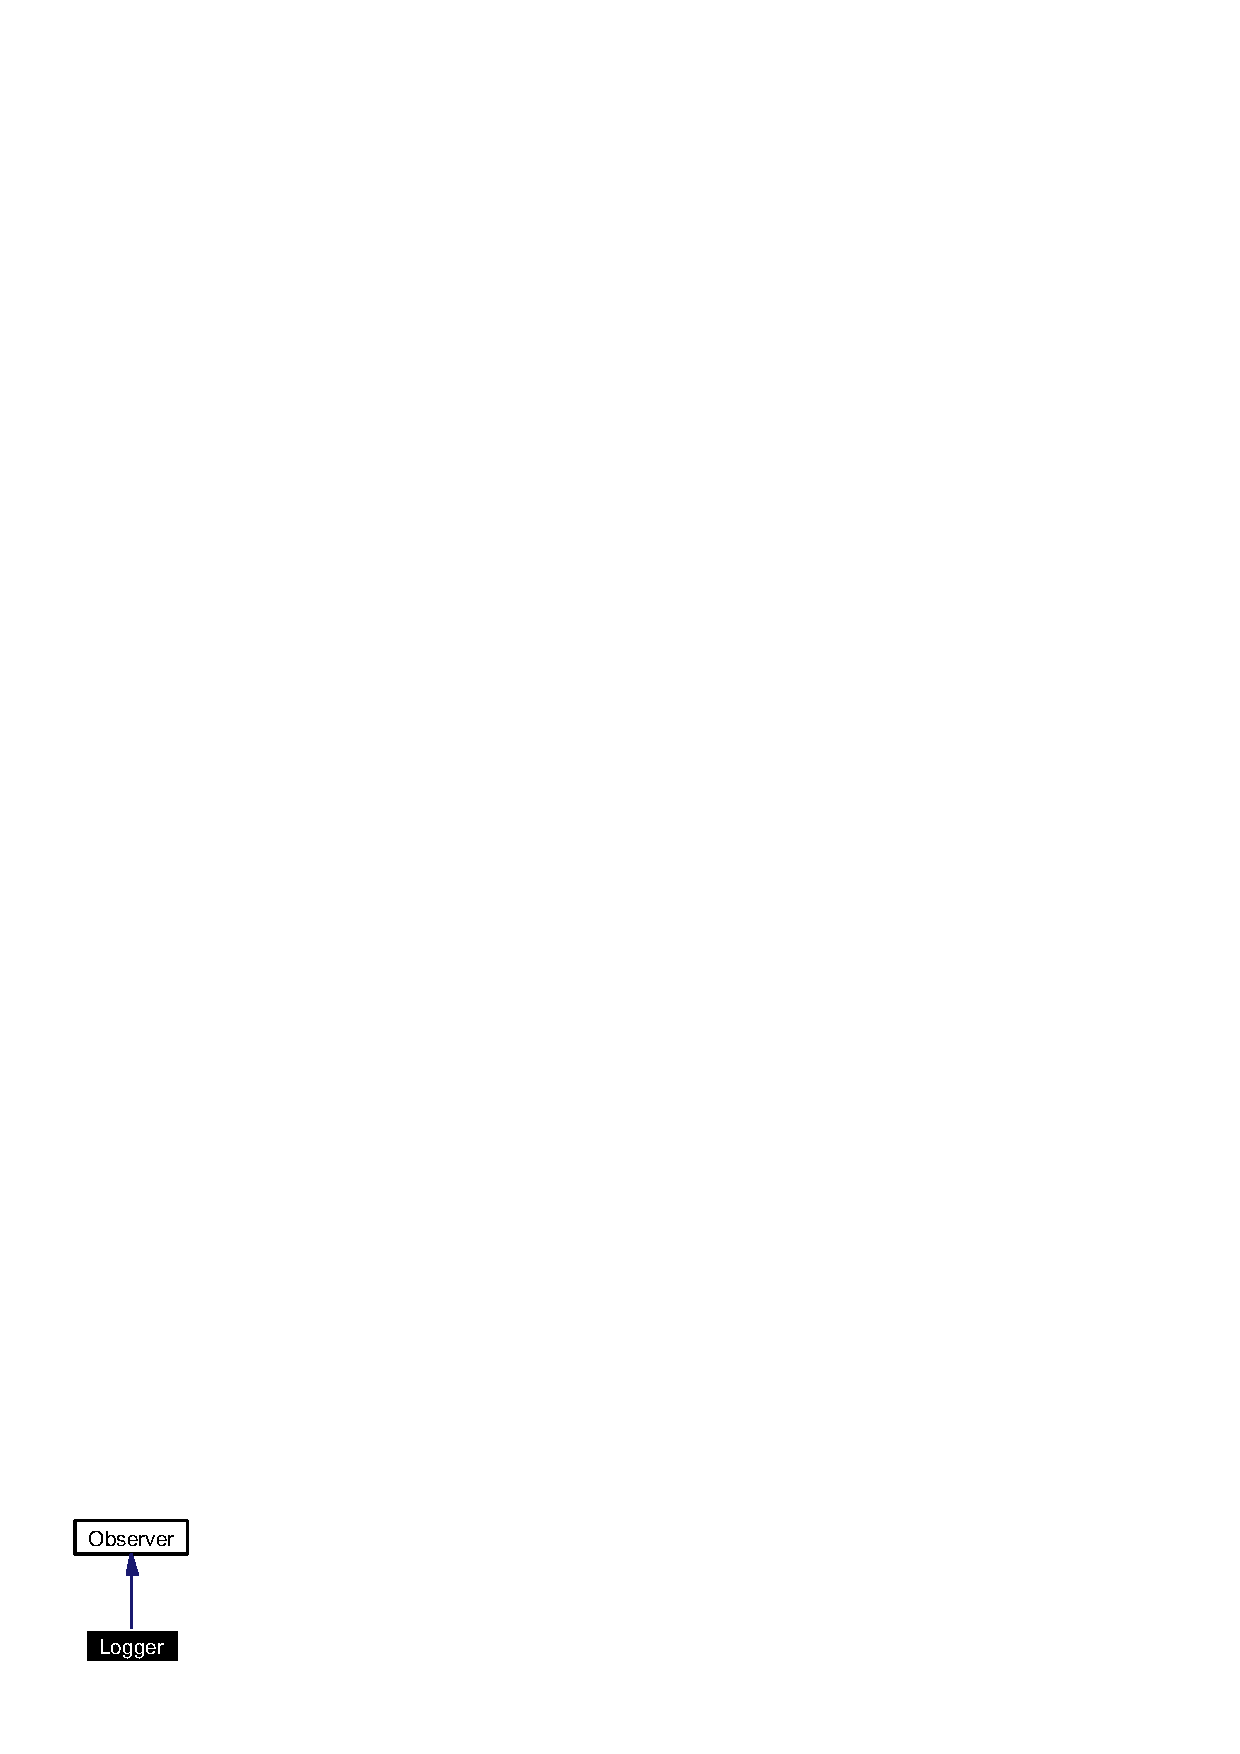
\includegraphics[width=45pt]{classLogger__coll__graph}
\end{center}
\end{figure}
\subsection*{Public Member Functions}
\begin{CompactItemize}
\item 
{\bf Logger} (\$filename)\label{classLogger_a0}

\item 
{\bf notify} (\$event, \$msg)\label{classLogger_a1}

\end{CompactItemize}
\subsection*{Public Attributes}
\begin{CompactItemize}
\item 
{\bf \$\_\-filename}\label{classLogger_o0}

\end{CompactItemize}


\subsection{Detailed Description}
blah.... 



Definition at line 9 of file Logger.php.

The documentation for this class was generated from the following file:\begin{CompactItemize}
\item 
Logger.php\end{CompactItemize}
